%%%%%%%%%%%%%%%%%%%%%%%%%%%%%%%%%%%%%%%%%%%%%%%%%%%%%%%%%%%%%%%%%%%%%%
% How to use writeLaTeX: 
%
% You edit the source code here on the left, and the preview on the
% right shows you the result within a few seconds.
%
% Bookmark this page and share the URL with your co-authors. They can
% edit at the same time!
%
% You can upload figures, bibliographies, custom classes and
% styles using the files menu.
%
% If you're new to LaTeX, the wikibook is a great place to start:
% http://en.wikibooks.org/wiki/LaTeX
%
%%%%%%%%%%%%%%%%%%%%%%%%%%%%%%%%%%%%%%%%%%%%%%%%%%%%%%%%%%%%%%%%%%%%%%
\documentclass{tufte-handout}

%\geometry{showframe}% for debugging purposes -- displays the margins

\usepackage{amsmath}
\usepackage[super]{nth}
% Set up the images/graphics package
\usepackage{graphicx}
\setkeys{Gin}{width=\linewidth,totalheight=\textheight,keepaspectratio}
\graphicspath{{graphics/}}

\title{Week 1 : An introduction to Python and Machine Learning\thanks{This document has been written in \LaTeX\ using the work of The Tufte-\LaTeX\ Developers which is Inspired by Edward~R. Tufte!}}
\author[Ramzi Saouma]{Ramzi Saouma}
%\date{}  % if the \date{} command is left out, the current date will be used

% The following package makes prettier tables.  We're all about the bling!
\usepackage{booktabs}

% The units package provides nice, non-stacked fractions and better spacing
% for units.
\usepackage{units}

% The fancyvrb package lets us customize the formatting of verbatim
% environments.  We use a slightly smaller font.
\usepackage{fancyvrb}
\fvset{fontsize=\normalsize}

% Small sections of multiple columns
\usepackage{multicol}

% Provides paragraphs of dummy text
\usepackage{lipsum}

% These commands are used to pretty-print LaTeX commands
\newcommand{\doccmd}[1]{\texttt{\textbackslash#1}}% command name -- adds backslash automatically
\newcommand{\docopt}[1]{\ensuremath{\langle}\textrm{\textit{#1}}\ensuremath{\rangle}}%optional command argument
\newcommand{\hlred}[1]{\textcolor{Maroon}{#1}}% prints in red
\newcommand{\docarg}[1]{\textrm{\textit{#1}}}% (required) command argument
\newenvironment{docspec}{\begin{quote}\noindent}{\end{quote}}% command specification environment
\newcommand{\docenv}[1]{\textsf{#1}}% environment name
\newcommand{\docpkg}[1]{\texttt{#1}}% package name
\newcommand{\doccls}[1]{\texttt{#1}}% document class name
\newcommand{\docclsopt}[1]{\texttt{#1}}% document class option name

\begin{document}

\maketitle% this prints the handout title, author, and date


\begin{abstract}
\noindent This course is about learning how to turn data into knowledge. While most of the cases and applications covered here focus on topics in finance and financial markets, the skills you acquire could be applied to other fields. The course is split into two parallel tracks. The first track revolves around learning the basics of Python. The second track centers around Machine Learning concepts and applications. During the first few weeks each track is taught separately. After the \nth{5} week, when enough material is covered from each track, the two tracks will coverage into one body of subjects.  (see figure~\ref{fig:syllabus}).
\end{abstract}
\begin{figure*}[h]%
  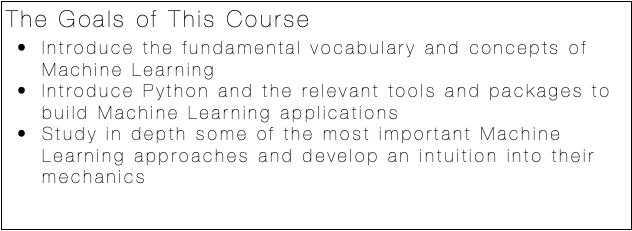
\includegraphics[width=\linewidth]{Goals.png}
  \caption{}
  \label{fig:packages}
\end{figure*}
\section{Python Basics}\label{sec:python-basics}
\subsection{Why Python?}\label{sec:why}
Python is relatively a young language. It only appeared in 1991 and over the last 10 years it became one of the predominant languages for data scientists. According to the Kaggle Machine Learning and Data Science  survey carried out in 2018, 83\% of respondents said that they used Python on a daily basis\footnote{\url{https://www.kaggle.com/sudhirnl7/data-science-survey-2018}}. While it is considered a scripting language \footnote{\hlred{Scripting Language}: a language that can be used quickly to automate small tasks. Typically scripting languages are not \hlred{compiled} but interpreted. Making them slower to run but faster and easier to write. }, it can be powerfull in building data applications. It is supported with an extensive body of data analysis libraries some of which we cover in this course. \\
On an entreprise level, many applications are initially developed by specialists using very \hlred{high level languages} \footnote{In comparison to \hlred{low-level languages}, a \hlred{high level language} is easier to use, it simplifies the interaction , making the process of developing a program  more accessible.}  such as R, SAS or Matlab as a proof of concept.At some point, when the application is ready for production it is rewritten in low level languages such as C++ or Java. What makes Python appealing to businesses is the fact that it can be an in-between language. It can be used for prototyping as well as for production. 
\subsection{Essential Python Libraries}\label{sec:libraries}

\begin{figure*}[h]%
  \includegraphics[width=\linewidth]{packages.jpg}
  \caption{List of pacakges}
  \label{fig:packages}
\end{figure*}






\newthought{NumPy} 
\\Numerical Python is considered the main library for numerical computing in \doccls{Python}. It provides efficient data structures(e.g \docopt{ndarray}), algorithims and library glue needed in most scientific applications involving numerical data in Python \cite{Mckinney2018}. NymPy will be covered in week 3.
\begin{figure*}[h]%
  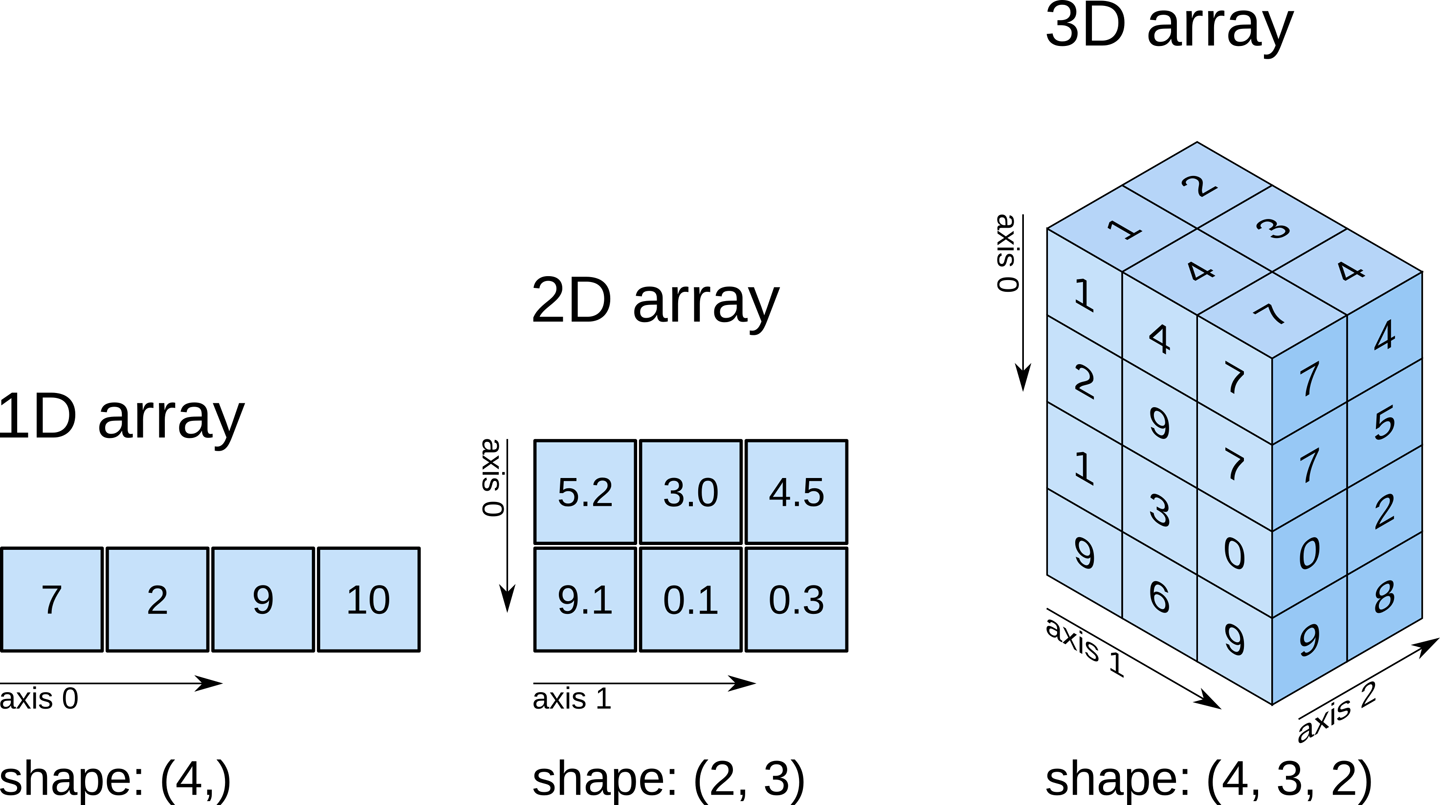
\includegraphics[width=\linewidth]{numpy.png}
  \caption{Numpy's ndarray illustrations}
  \label{fig:packages}
\end{figure*}

\newthought{pandas}
\\ Pandas offers a high level data structures and functions designed to facilitate the work of data scientist. It is built around a data structure called the DataFrame that is inspired from the R DataFrame.  Looking like an Excel spreadsheet, it is effectively a table filled with data. Pandas provides a great range of methods to modify and operate on the table. In contrast to NumPy, which requires that all entries in an array be of the same type, pandas allows each column to have a separate type. Another great advantage of pandas is its ability to import from a great variety of file formats and databases.
\begin{figure*}[h]%
  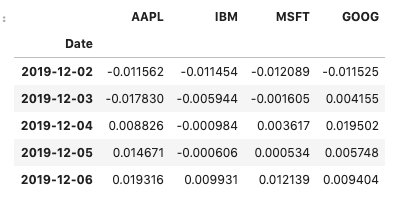
\includegraphics[width=\linewidth]{pandas.png}
  \caption{Pandas's DataFrame example}
  \label{fig:packages}
\end{figure*}
\begin{figure*}[h]%
  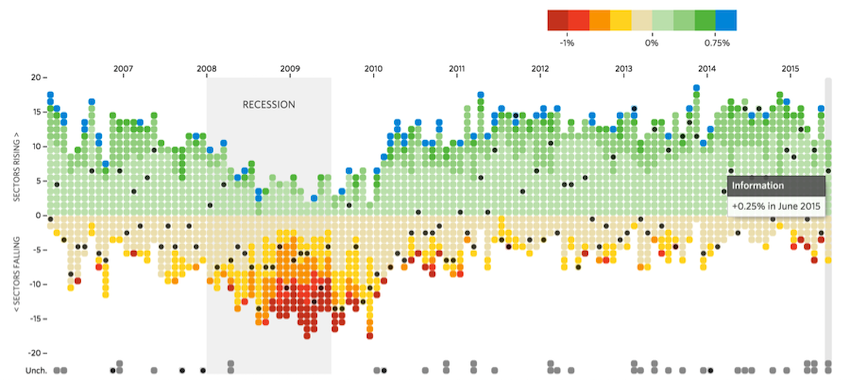
\includegraphics[width=\linewidth]{matplotlib.png}
  \caption{Matplotlib example}
  \label{fig:packages}
\end{figure*}
\begin{figure*}[h]%
  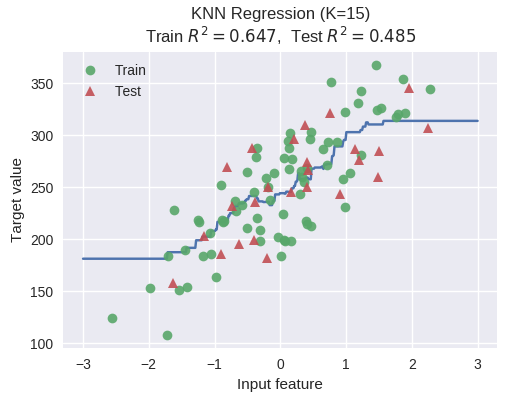
\includegraphics[width=\linewidth]{sclearn.png}
  \caption{ScKit-Learn powerfull Machine Learning functionalities}
  \label{fig:packages}
\end{figure*}
\newthought{matplotlib}
\\matplotlib is the main and most widely used visualization library in Python. It offers functions for making high-quality visualizations such as line charts, histograms, scatter plots. Visualizing your data and different aspects of your analysis can give you important insights, and we will be using matplotlib for all our visualizations. The high quality and versatility of the graphs makes it a great tool to present your findings as well.


\newthought{SciPy}
\\SciPy is a collection of functions for scientific computing in Python. It provides, among other functionality, advanced linear algebra routines, mathematical function optimization, signal processing, special mathematical functions, and statistical distributions. scikit-learn draws from SciPy’s collection of functions for implementing its algorithms.


\newthought{scikit-learn}
\\scikit-learn is an open source project, meaning that it is free to use and distribute, and anyone can easily obtain the source code to see what is going on behind the scenes. The scikit-learn project is constantly being developed and improved, and it has a very active user community. It contains a number of state-of-the-art machine learning algorithms, as well as comprehensive documentation about each algorithm. scikit-learn is a very popular tool, and the most prominent Python library for machine learning. It is widely used in industry and academia, and a wealth of tutorials and code snippets are available online. scikit-learn works well with a number of other scientific Python tools, which we will discuss later in this chapter \cite{Muller2017}.





\subsection{Installing Python}

The most commonly used free package to install Python is Anaconda distribution For the sake of the course we would be using Python 3.6. This could be found at (\url{http://anaconda.com/downloads}).

\newthought{windows}- To test if the application is configured properly, open the command prompt (cmd.exe) and try to lunch the interpreter by typing \docenv{python}. 
\begin{docspec}
\url{C:/Users/wesm/python}
\\Python 3.7.1 |Anaconda 4.1.1 (64-bit)| (default, Jul 5 2016, 11:41:13)
\\[MSC v.1900 64 bit (AMD64)] on win32
\\> > > 
\end{docspec}
To exit shell type \docenv{exit()}
\newthought{Apple(os x, macOS)} - To test if the application is setup properly, type \docenv{\$ python}
\begin{docspec}
\\ Python 3.7.1 (default, Dec 14 2018, 13:28:58) 
\\ [Clang 4.0.1 (tags/RELEASE \_ 401/final)] :: Anaconda, Inc. on darwin.
\\ Type "help", "copyright", "credits" or "license" for more information.
\\> > > 
\end{docspec}
To exit shell type \docenv{exit()}

\subsection{IPython and Jupyter}
IPython is a 'command-line based' application that allows better interactive Python interpreter. It is based on he idea of \docopt{execute-explore}  workflow instead of the  \docopt{edit-compile-run} workflow which is common to other languages. 
In recent times, the developers of  IPython launched a new interactive, language agnostic application the \doccls{Jupyter Notebook}.
The \doccls{Jupyter Notebook} is increasingly becoming popular by being adopted as he main platform for data scientists. It is a very powerful tool to use in the classroom, to develop teaching materials and to share lessons and tutorials.The Jupyter Notebook is an interactive environment for running code in the browser. It is a great tool for exploratory data analysis. While the Jupyter Notebook supports many programming languages, we only need the Python support. The Jupyter Notebook makes it easy to incorporate code, text, and images. 
\section{Machine Learning: The Anti-Spam Case}

\textbf{\hlred{Machine Learning is the systematic study of algorithms and systems that improve their knowledge or performance with experience}}\cite{Flach2012}

This case is copied from chapter 1, 'Ingredient of machine learning', of Peter Flach's book. The goal is to get familiarized with some basic concepts and definitions. Every time a new concept is introduced, i will explicitly explain the definition on the right hand side of the documents with the concept written in red color.

On daily basis we receive and send emails. Most of the email providers equip our inbox with some sort of a spam filter. You might not be aware, but anti-spam filters rely heavily on machine learning. In fact most of them rely on 'SpamAssasin'\footnote{\url{https://spamassassin.apache.org}} which is an open-source spam filter. 
It uses a scoring algorithm that integrate a wide range of advanced heuristic and statistical analysis tests on email headers and body text. Every test produces a score and if the total score is higher than 5 the email is classified as spam. It is worth noting that some tests could produce negative scores as well.


\subsection{How to Build A Spam Filter?}
Suppose we want build a Spam filter. We will need a large \hlred{training set}\footnote{A \hlred{training data} set in machine learning is the actual data input used to train the model for performing various tasks. } of emails which have been manually labelled spam or non-spam. Hence for these emails we already know the results of all the tests we would like to introduce. Our initial goal  is to come up with a weighting system to apply on those tests, such as when all scores are added the spam emails get 5 or more as a score. 
\begin{table}[ht]
  \centering
  \fontfamily{ppl}\selectfont
  \begin{tabular}{lllll}
    \toprule
    Email & x_{1} & x_{2} & Spam? & 4x_{1} + 4x_{2}\\
    \midrule
    1 & 1 & 1 & 1 & 8 \\
    2 & 0 & 0 & 0 & 0 \\
    3 & 1 & 0 & 0 & 4 \\
    4 & 0 & 1 & 0 & 4 \\

    \bottomrule
  \end{tabular}
  
  \caption{With training data set of 4 emails, the results of two tests are denoted by x and x. Knowing that 1 is spam we opt for the weights 4 and 4. The results seems to be producing the desired outcome. Email 1 scores 8 (higher than 50 while the non spam emails score less than 5.}
  \label{tab:normaltab}
%\zsavepos{pos:normaltab}
\end{table}
To keep it simple, lets say we have two tests and four emails in our training data. Based on the data we have both tests succeed for email 1, which has been hand labelled as spam. It is easy to see that assigning the weights 4 for each test will produce the desired outcome. In fact any weights between 2.5 and 5 can produce the desired results. 
If you are wondering how this classification problem is related to learning, your are not wrong. In fact the only reason why we call it learning is because the more examples and counter examples we give our model the better our classifier will be. The concept of \textbf{improving performance with experience} is central to machine learning and it ties up nicely with the definition we presented at the beginning of this section. In practice experience refers to our training data set and performance refers to its ability to filter out spam emails.
\begin{figure*}[h]%
  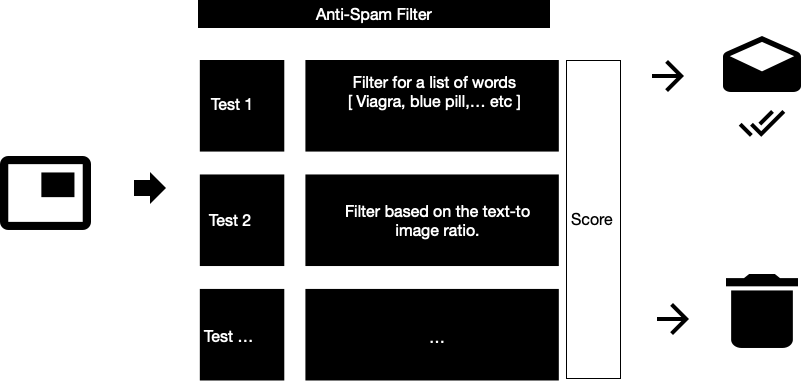
\includegraphics[width=\linewidth]{antispam.png}
  \caption{Anti-Spam filter}
  \label{fig:packages}
\end{figure*}
One important fact to note, is that when we talk about performance we are referring to the emails we are going to receive in the future and are going to be filtered correctly. We don't care so much about the performance of the model on the training data. We already know which email are spam!
While it is important to have good performance on the training data, this remains just a mean to an end. In fact trying to hard to achieve good performance on training data could lead to another problem which is \hlred{overfitting}\footnote{\hlred{Overfitting} is a problem that occurs when we fit the model to close to the training data. This leads to a failure in being able to generalise the model for future observations.}.
\newthought{Generalisation} is the core principle of machine learning. If we fail to generalize the knowledge that the spam filter learned to future incoming email we then have another problem to solve. If it is not overfitting it could be that the data doesn't represent the user's preference and behaviour. This problem is also known as \hlred{underfitting} \footnote{\hlred{Underfitting}  occurs when a model is too simple — informed by too few features or regularized too much}. If that is the source of the problem, machine learning could adapt to the behaviour and preferences of the user. It could as well be that the linear classification we defines by \ 4x_{1} + 4x_{2} \] is bigger than 5 is not correct. Furthermore we have not talked about test  themselves yet. What if the tests are not ideal or perhaps more tests are needed? Indeed how do we come up with those tests? Spam assassin uses several tests which for example include the text-to-image ratio test. Moreover Spam assassin scans the content of the email for words and phrases that increases or decreases the chances of the email to be spam. Surely words like "Viagra" or sentences such as 'confirm your account details' will increase the chances of the email being a spam. This type of test uses the text \hlred{classification} \footnote{\hlred{Classification} has the goal to predict a class label for a list of possibilities. In the current AntiSpam case we are dealing with two classes.} techniques. Those tests store large dictionaries of words and sentences that are potential spam. For each of those words a certain probability of spam/not-spam is maintained. The probabilities are derived from the training data. 
Assume 5 emails in the training data has the word 'Viagra' and 4 out of five emails were tagged as spam, then the probability of an new email being a spam given the occurrence of the word 'Viagra' is then 80\%.

%\printclassoptions





\begin{marginfigure}%
  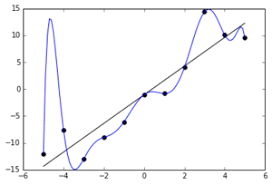
\includegraphics[width=\linewidth]{overfitting.png}
  \caption{Example of overfitting from Wikipedia. A simple straight line is a better fit than the the complex blue line. }
  \label{fig:marginfig}
\end{marginfigure}


\begin{marginfigure}%
  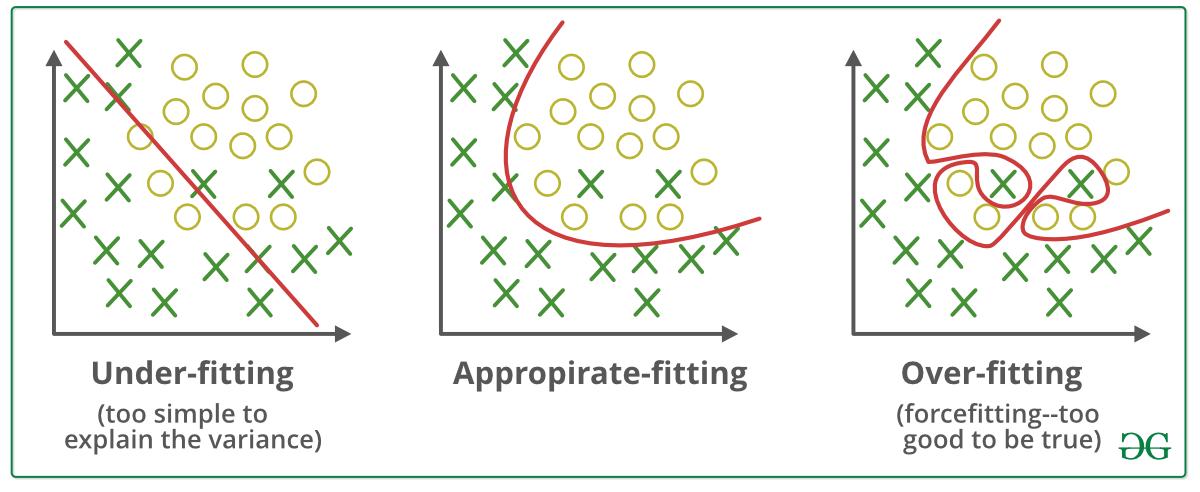
\includegraphics[width=\linewidth]{fitting.png}
  \caption{Generalisations of a classifier. source:www.geeksforgeeks.org/}
  \label{fig:marginfig}
\end{marginfigure}



But this is not the whole story because we have to take into account the prevalence of spam. Suppose we receive on average one spam e-mail for every six non-spam e-mails . This means that I would estimate the odds of the next e-mail coming in being spam as 1:6. If after that we spot the word ‘Viagra’ is in the text, we need to adjust for the initial probability by combining the two together. According to \hlred{Bayes'} \footnote{\hlred{Bayes' Rule}: "Suppose you throw a pair of standard dice. The probability that the total is 10 is \(\frac{1}{12}\) because there are thirty-sex ways the dice can come up, of which three(4 and 5, 5 and 5, and 6 and 4) give 10. If, However, you look at the first die and see that it came up as 6, then the conditional probability that the total is 10, given this information, is \(\frac{1}{6}\)   (since that is the probability that the other die comes up as 4).  In general, the probability of A given B is defined to be the probability of A and B divided by the probability of B. In symbols:"\[ P[A \mid B]=\frac{P[A \wedge B] }{P[B]}\] From which we derive a more interesting formula:
\[ P[A \mid B]=\frac{P[A \mid B]P[A] }{P[B]}\] \cite{Gowers2008}} rule to get the joint probability we should multiply them: 1:6 times 4:1 is 4:6, corresponding to a spam probability of 40\%. Hence, despite the  of the word ‘Viagra’, the safest bet is still that the e-mail is ham, which does not sound very intuitive.

\begin{marginfigure}%
  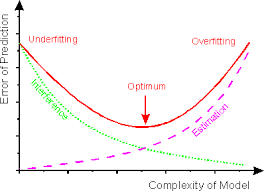
\includegraphics[width=\linewidth]{tradeofffitting.png}
  \caption{The trade-off between complexity and accuracy}
  \label{fig:marginfig}
\end{marginfigure}
\begin{marginfigure}%
  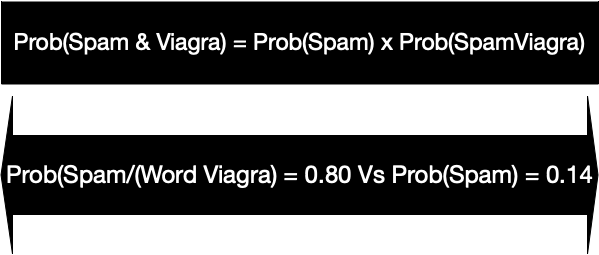
\includegraphics[width=\linewidth]{Bayes.png}
  \caption{Bayes Rule at play}
  \label{fig:marginfig}
\end{marginfigure}
The way to make sense of this is to realise that you are combining two independent pieces of evidence, one concerning the prevalence of spam, and the other concerning the occurrence of the word ‘Viagra’. These two pieces of evidence pull in opposite directions, which means that it is important to assess their relative strength. What the numbers tell you is that, in order to overrule the fact that spam is relatively rare, you need odds of at least 6:1. ‘Viagra’ on its own is estimated at 4:1, and therefore doesn’t pull hard enough in the spam direction to warrant the conclusion that the e-mail is in fact spam. What it does do is make the conclusion ‘this e-mail is not spam’ a lot less certain, as its probability drops from 6/7 = 0.86 to 6/10 = 0.60.
The nice thing about this ‘Bayesian’ classification scheme is that it can be repeated if you have further evidence. For instance, suppose that the odds in favour of spam associated with the phrase ‘blue pill’ is estimated at 3:1 (i.e., there are three times more spam e-mails containing the phrase than there are ham e-mails), and suppose our e- mail contains both ‘Viagra’ and ‘blue pill’, then the combined odds are 4:1 times 3:1 is 12:1, which is ample to outweigh the 1:6 odds associated with the low prevalence of spam (total odds are 2:1, or a spam probability of 0.67, up from 0.40 without the ‘blue pill’).
That was a quick peek into what is commonly know at the Naive Bayesian Classifier. This is one of the dozen of algorithms we are going to cover in this course. Machine learning is all about designing the right \hlred{features} to construct the right \hlred{models} that achieve the desired \hlred{tasks}. In the anti-spam case we used the appearance of words like "Viagra" and "Blue pill" as \hlred{features} in the content of an email while applying the Naive Bayesian algorithm to build a \hlred{model} that has the \hlred{task} to filter our spam emails. 
%\begin{figure*}[h]%
%  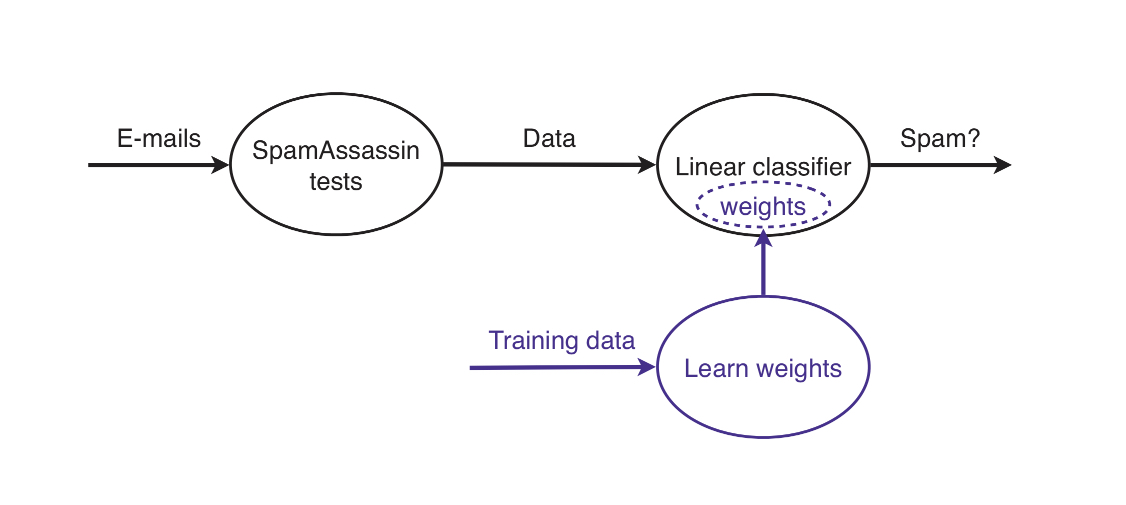
\includegraphics[width=\linewidth]{Spam_g1.jpeg}
% \caption{At the top we see how SpamAssasin approaches the spam email classification task: the text of each email is converted into a data point by means of SpamAssasin's built-in tests, and a linear classifier is applied to obtain a spam or a non-spam decision. }
%  \label{fig:marginfig}
% \end{figure*}
%%%%




\section{Categories of Machine Learning}\label{sec:python-basics}

\begin{figure*}[h]%
  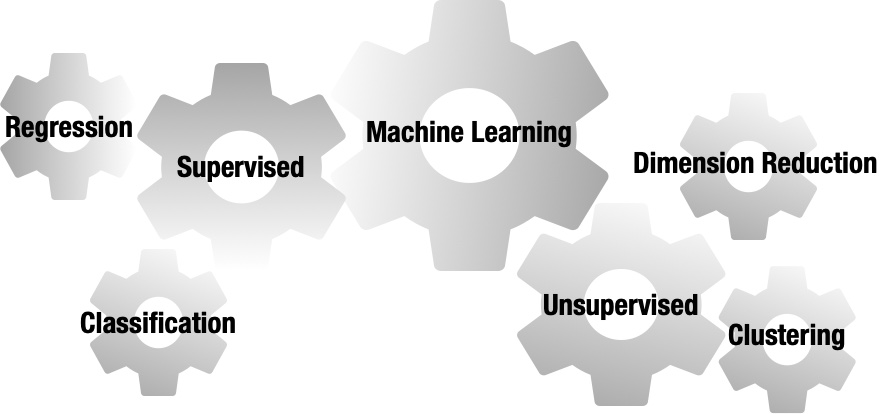
\includegraphics[width=\linewidth]{Categories.jpg}
  \caption{The Machine Learning Universe.}
  \label{fig:syllabus}
\end{figure*}


\\At the most basic level, machine learning can be divided into two main categories: \hlred{supervised} learning and \hlred{unsupervised} learning.
"Supervised learning involves somehow modeling the relationship between measured features of data and some label associated with the data; once this model is determined, it can be used to apply labels to new, unknown data."\cite{Vanderplas2017}. Furthermore Supervised learning could be subdivided into classification tasks and \hlred{regression}\footnote{\hlred{Regression} analysis is a set of statistical processes for estimating the relationships between a dependent variable (often called the 'outcome or target variable') and one or more independent variables (often called 'predictors' or 'features')} tasks: in classification, the labels are discrete categories or classes, while in regression, the labels are continuous numbers or quantities. 
"Unsupervised learning involves modeling the features of a data set without reference to any label, and is often described as “letting the data set speak for itself.” These models include tasks such as \hlred{clustering} and \hlred{dimensionality} reduction" \cite{Vanderplas2017}. Clustering algorithms arranges data into similar groups, while dimensionality reduction tend to simplify the features by reducing them into main drivers and factors. 

\subsection{Supervised Learning: Classification}
\begin{figure*}[h]%
  \includegraphics[width=\linewidth]{Classification.png}
  \caption{An abstract visualisation of a two features binary classification}
  \label{fig:Class}
\end{figure*}

\begin{figure*}[h]%
  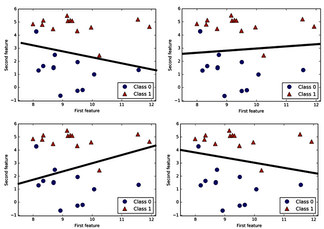
\includegraphics[width=\linewidth]{Classification_1.png}
  \caption{Separating the two classes with a straight line}
  \label{fig:Class}
\end{figure*}


We start with an abstract classification, where based on two features we want to be able to classify an input between two classes. Here we have a 2-dimensional data set which is used to \hlred{train} the model. In addition we have two classes represented by different colors/shape on the graph. 
\\There are a many possible ways to model this classification task, but we will start by adopting a fairly simple one. It is based on the assumptions that the two classes can be separated by drawing a straight line through the plane between them, such that points on each side of the line fall in the same group. Looking at figure 13, by just using rough visual estimations we can potentially draw several acceptable separation lines. In this case the model \hlred{parameters} are the particular numbers describing the slope and intersection of that line for our data. Which line to opt for is learned from the data, which is often called training the model.
Now that this model has been trained, it can be generalized to new, unlabeled data. In other words, we can take a new set of data, draw this model line through it, and assign labels to the new points based on this model. This stage is usually called prediction.

This reminds us of the previous of anti-spam filtering for email; in this case, we might use the following features and labels:
\begin{enumerate}
    \item feature 1, feature 2, etc.: counting of key terms (“Viagra,” “blue pill,” etc.)
    \item labels:   “spam” or “not spam”
\end{enumerate}

For the training set, these labels might be determined by individual inspection of a small representative sample of emails; for the remaining emails, the label would be determined using the model. For a suitably trained classification algorithm with enough well-constructed features (typically thousands or millions of words or phrases), this type of approach can be very effective. 

\subsection{Supervised Learning: Regression}

\begin{figure*}[h]%
  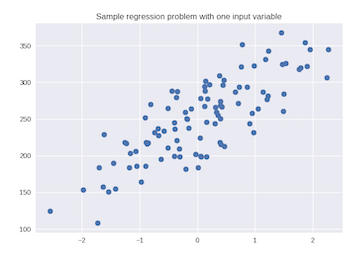
\includegraphics[width=\linewidth]{regression.png}
  \caption{1 Dimensional simple data set for regression}
  \label{fig:syllabus}
\end{figure*}
\begin{figure*}[h]%
  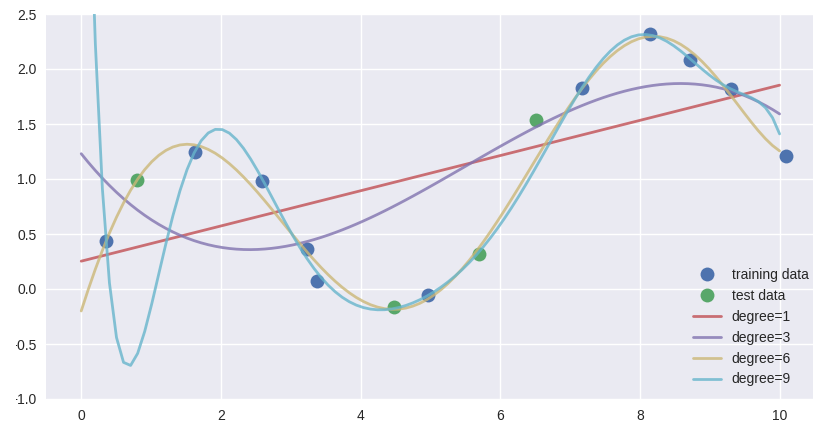
\includegraphics[width=\linewidth]{regression_1.png}
  \caption{Regression fitting}
  \label{fig:syllabus}
\end{figure*}
In contrast with the discrete labels of a classification algorithm, we will next look at a simple regression task in which the labels are continuous quantities. On the x-axis we have one feature that varies between -2 and +2 and we aim to use it to predict the y-axis. The most basic and simple algorithm is to apply is the old linear ordinary least square  linear regression. But in this course will be visit more elaborate and complex algorithms to fit a line into a continuous data target.

In the figure 15 you see 4 different fitting lines into a different data set. We start from the simplest linear regressions(red) to the most complex overfitted non-linear curve (light blue). Again the model parameters in this case are he slope and the intersection of the lines. 

The type of tasks to which we apply regressions is extremely vast. This could be applied to predicting the level of inflation in an economy based on certain levels of other economic indicators:
\begin{enumerate}
    \item feature 1, feature 2, etc.: year-to-date average unemployment,interest rates, etc.)
    \item labels:  the level of inflation.
\end{enumerate}



\subsection{Unsupervised Learning: Clustering}

The classification and regression example we considered cases of supervised learning algorithms, in which we our goal is to build a model that will predict labels for new data. Unsupervised learning involves models that describe data without reference to any known labels.
One common case of unsupervised learning is “clustering,” in which data is automatically assigned to some number of discrete groups. For example, we might have some two-dimensional data like that shown in Figure 16.

\begin{figure*}[h]%
  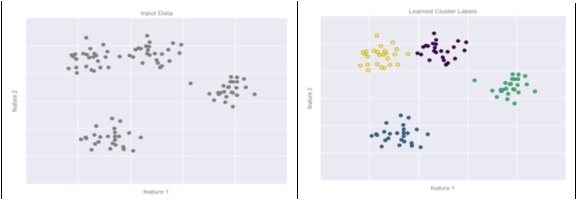
\includegraphics[width=\linewidth]{clustering.jpg}
  \caption{Clustering example}
  \label{fig:clustering}
\end{figure*}

Contemplating the plot on the left hand side, it is clear that each of these points is part of a distinct group. We can discern 3 or maybe 4 different groups. Based on the features' input, a clustering algorithms will model the intrinsic structure of the data to determine which points could be clustered within the same group. A very fast and intuitive algorithm, known as  \hlred{k-means}\footnote{\hlred{K-Mean} fits a model consisting of k cluster centers; the optimal centers are assumed to be those that minimize the distance of each point from its assigned center. Again, this might seem like a trivial exercise in two dimensions, but as our data becomes larger and more complex, such clustering algorithms can be employed to extract useful information from the data set.
We will discuss the k-means algorithm in more depth} algorithm, is applied and the output is seen on the right hand side of the figure where each color corresponds to a different cluster.
There is a multitude of application for clustering algorithms. Companies use clustering to categories their clients and use the output while designing their marketing or sales strategy. The features could be anything from client's income to spending habits. 

\subsection{Unsupervised Learning: Dimensionality reduction }
In dimensionality reduction we aim at inferring a structure from looking at the data. As a method is a bit more abstract than the examples we looked at before, but generally it seeks to pull out some low-dimensional representation of data that in some way preserves relevant qualities of the full dataset. Principle component analysis (PCA) is one example of dimensionality reduction. PCA is a statistical method that applied an orthogonal transformation to convert a the data set possibly correlated features into a lower set of values of linearly uncorrelated variables called principal components. We will revisit this with more concrete examples later in the course. Once common use is when we are dealing with the large number of features that we suspect to be correlated. Dimensionality reduction has a lot of advantages especially when it comes to visualisation. Being able to explore a data set visually if it is 2 dimensional rather than 10 is powerful. 

\section{Summary}

So far we have seen a few intuitive examples of some of the basic types of machine learning approaches. Obviously, we have just touched the surface of those methods, but I hope this section was enough to give you a basic idea of what types of problems machine learning approaches can solve.
To summarize:
\newthought{Supervised learning}
\\Models that can predict labels based on labeled training data
\newthought{Classification}
\\Models that predict labels as two or more discrete categories
\newthought{Regression}
\\Models that predict continuous labels
\newthought{Unsupervised learning}
\\Models that identify structure in unlabeled data
\newthough{Clustering}
\\Models that detect and identify distinct groups in the data
\newthought{Dimensionality reduction}
\\Models that detect and identify lower-dimensional structure in higher- dimensional data

\bibliography{sample-handout}
\bibliographystyle{plainnat}
\end{document}

